\chapter{Implementation}
\label{chap:impl}
This chapter is dedicated to report the implementation of our genealogy management program.
Firstly, we present a specification for our new programming language named \textbf{KISP}:
\textbf{K}inship LI\textbf{SP}. Secondly, we describe the overall structure of the program, including its three major components:
Database Manager, Virtual Assistant and KISP Interpreter.

\section{KISP Language Specification}
\subsection{Grammar and Lexical Structure}
    Since KISP is a dialect of LISP, it inherits some syntax from the predecessor, but generally it is a new programming language. The
    grammar is presented with the help of Bacus-Naur notational technique. For the sake of simplicity we omit angle brackets and
    embolden non-terminal words. A plus, a star sign in a superscript and a question mark have the same meaning as in regular
    expressions.
    \begin{align*}
        \text{\textbf{term}} &::= \text{\textbf{literal}} | \text{\textbf{lambda}} | \text{\textbf{define}} | \text{\textbf{atom}} |
            (\text{\textbf{term}}^+) \\
        \text{\textbf{lambda}} &::= (\text{lambda (\textbf{reference}}^*\text{) \textbf{term}}) \\
        \text{\textbf{define}} &::= ( \text{define \textbf{reference} \textbf{term}}) \\
        \text{\textbf{reference}} &::= \text{\textbf{word}\{-\textbf{word}\}'?'?} \\
        \text{\textbf{word}} &::= \text{\textbf{letter}}^+ \\
        \text{\textbf{letter}} &::= a | b | ... | z | A | B | ... | Z \\
        \text{\textbf{atom}} &::= * | + | \text{concat} | \text{list} | \text{append} | ... \\
        \text{\textbf{literal}} &::= \text{void} | \text{true} | \text{false} | \text{people} | \text{vacant} | \text{now} |
            \text{\textbf{numeral}} | \text{\textbf{string}} \\
        \text{\textbf{numeral}} &::= \text{-?\textbf{digit}}^* \\
        \text{\textbf{digit}} &::= 0 | 1 | ... | 9 \\
        \text{\textbf{string}} &::= `\text{\textbf{symbol}}^*` \\
        \text{\textbf{symbol}} &::= \text{\textit{any non-blank ASCII symbol}}
    \label{al:bnf}
    \end{align*}
    As we can see from the definition, there are three kinds of terminals in the grammar: literals, references and atom functions,
    which are called simply \textbf{atom}s. Literals are instances of primitive types, such as \textit{Numeral}, \textit{String} or
    \textit{Boolean}, or special keywords. They stands for the following: "void" represents NULL type, "people" -- a list of
    all persons in a family tree, "now" -- the current time entry and "vacant" -- an empty list. References are used as definientia in
    "define" terms and as names for parameters in lambda terms. It is possible for a reference to end in a question mark, which means
    that it denotes an instance of \textit{Boolean} type. References can we written in so-called \textit{dash case}, so "long-name"
    and "very-long-name" are both legal. The only exception are names which start with the dash like "-illegal", they are invalid.

    Note that we allow niladic lambdas, so, for instance, this is a valid expression: \texttt{(lambda () 'Hello, World!')}. But at the
    same time \texttt{()} is not a well-formed term. We also prohibit "define" terms inside other terms, so this would not work:
    \texttt{(+ 2 (define three 3))}. Strings are nested in single quotes, integers, in KISP we call them "numerals", can start with a
    zero and be prefixed by a negative sign.

    Here is the complete list of all keywords in KISP: \textbf{true}, \textbf{false}, \textbf{define}, \textbf{lambda},
    \textbf{people}, \textbf{now}, \textbf{void}, \textbf{if}, \textbf{vacant}. The rule is that you can use as a reference everything
    you want as long as it is not a keyword, so you cannot redefine their standard behaviour, thus a programmer is unable to tamper
    with inner workings of the interpreter.

    As in all other dialects of LISP, a term \texttt{(f a b c ...)} means the \textit{execution} of a function $f$ with the
    specified arguments $f(a, b, c, ...)$. Of course, we can construct and call the higher-order functions as usual:
    \texttt{((twice square) 2)} will yield $16$, or \texttt{((compose inc inc) 0)} which prints $2$.

    Recursion also works as in any other LISP-like language. For example, here is the function that computes the $n$-th term of
    the famous Fibonacci sequence:
    \begin{verbatim}
    (define fibonacci
        (lambda (n)
            (if (< n 2)
                1
                (+ (fibonacci (- n 1)) (fibonacci (- n 2)))
            )
        )
    )
    \end{verbatim}
    However, using a reference before its definition is prohibited. For instance, the following code would not execute:
    \begin{verbatim}
    (+ 1 two)
    (define two 2)
    \end{verbatim}
    The interpreted will fail to recognize "two" as a valid reference in the first term and therefore will print an error message.
    The same applies to references in "define" term: cyclic definitions are forbidden:
    \begin{verbatim}
    (define zero (prev one))
    (define one (succ zero))
    \end{verbatim}

\subsection{Data Types}
    There are eight data types in KISP, four primitive and four composite. Primitive types: \textit{Boolean}, \textit{Numeral},
    \textit{Void} and \textit{String}. Composite: \textit{Function}, \textit{List}, \textit{Person} and \textit{Date}. An instance of
    a primitive type can be obtained by a literal, whereas a composite object is created only through calling a corresponding
    \textit{constructor} function. For instance, to make a list of three numbers one should use the following term: \texttt{(list 0 1
    2)}. However, there are three pre-defined global constants of composite types: \textit{now}, \textit{vacant} and \textit{people}.

    KISP is a \textit{dynamically} typed program language, which meas that information about a type of an entity is present only at
    execution time. This approach has certain benefits over \textit{static} typing as well as some disadvantages.

    For each type there are corresponding atomic functions provided by default to work with that type. Here we will present the atomic
    functions only for the type \textit{Person}, since it is the main element that distinguish KISP from other dialects. For the full
    documentation of other functions one can refer to the Appendix C\ref{chap:doc}.

    In order to create an instance of the type \textit{Person}, one should write \texttt{(person 'full name')}. This function will
    look up and return a person with stated full name in a linked family tree, or "void" if there is no person with such name.
    This function also has the following form: \texttt{(person 'first name' 'last name')}. All arguments are case-insensitive.

    The function \texttt{kinship} provides a convenient way to ascertain how a person $p_1$ is related to the person $p_2$:
    \texttt{(kinship $p_1$ $p_2$)}. It returns a \textit{list} of basic kin terms as strings. The content of such
    list corresponds exactly to a composite kinship term describing the relation of $p_1$ and $p_2$ to each other. For example, let us
    assume that there are two persons in our family tree: Alice and Bob. Alice is a niece of Bob, so if we to evaluate the term
    \texttt{(kinship (person 'alice') (person 'bob'))} we would get a term which is equal to \texttt{(list 'daughter' 'parent' 'son')}.
    The result can also be empty, but only if two persons are not related at all, i.e. the family tree has multiple connected components.

    In order to reduce a long kinship term generated by the latter method, one can use \textit{shorten} function that accepts the list
    of basic kin terms and performs the reduction algorithm outlined in the listing \ref{algo:red}. Using the previous example, running
    \texttt{(shorten (kinship (person 'alice') (person 'bob')))} will yield to the list of exactly one element: "niece". This function
    can be of use when printing the result of \textit{kinship}.

    Another useful function which return a specified attribute of a person is \textit{attr}. Here is how we can get a persons
    birthday: \texttt{(attr person 'birthday')}. This term produces the date of birth of a \texttt{person} as an object of type
    \textit{Date}. The list of all attributes accepted by \textit{attr} can be found in the full documentation \ref{doc:attr}.

    Of course, there are unitary functions corresponding to the denotations of basic kin terms: \textit{mother}, \textit{father},
    \textit{spouse} and \textit{children}. Here is how we can get a \texttt{person}s paternal grand-mother: \texttt{(mother (father
    person))}. All those functions return a list of respective relatives/in-laws. This list can be empty iff there is no such relative
    present in a family tree.

    Another interesting function is \textit{gen-dist}, which calculates the \textit{generational distance} between two persons.
    The distance $d$ is defined as the number of the level of the second person \textit{relative} to the first, where the level of the
    second person is considered to be zero:
    \begin{itemize}
        \item{The distance is a symmetric function: $d(x, y) = d(y, x)$, for all $x$ and $y$.}
        \item{It is zero for every two individuals from the same generation, including the person himself: $d(x, x) = 0$.}
        \item{Father located on the previous level, so $d(x, father(x)) = -1$.}
        \item{On the other hand, child inhabits the next level, thus $d(child(x), x) = 1$, and so on.}
    \end{itemize}
    For $d$ the calculation process is to start with zero, then increment each time we descend one level and decrement every time we
    ascend a level.

    The last function in the repertoire of the \textit{Person} type is \textit{put-kinship}. It is used to append a new entry
    into the $\omega$ dictionary, thus enhancing the capabilities of \textit{shorten}. For example, with \texttt{(put-kinship
    'son,parent,parent' 'uncle')} we can reduce avuncular terms. To correctly specify the formal kinship term, one must follow strict
    guidelines:
    \begin{enumerate}
        \item{Use only nine basic kinship terms.}
        \item{Separate them with a single comma without any in-between spaces.}
    \end{enumerate}

\section{System Structure}
    % User requirements!!!
    % Если что спросят про bonds, просто сказать что в требованиях такого функционала не было.
    Firstly, we shall determine the user requirements for our program. Since there was no individual customer, who would say what
    features are indispensable and what are superfluous, we had to play this role ourselves. That eliminated the potential problems
    which one can encounter when trying to understand the needs of the user. Also, by putting ourselves into the situation of a
    potential customer, who often has rather trivial knowledge of IT, we gained an understanding of his point of view, which will be
    particularly helpful to us later.

    After careful considerations, we arrived at the following list of requirements:
    \begin{enumerate}
        \item{A user must be able to see his carefully crafted family tree in a nice visualisation.}
        \item{A user wants to move and scale this visualisation.}
        \item{A user must have an ability to move the nodes of his family tree.}
        \item{A user wants to add and remove members of his family.}
        \item{A user must be able to link his relatives together with nuptial and parental bonds.}
        \item{A user must be able to edit the profile of a person in his genealogy.}
        \item{A user must have an ability to manage many genealogies without losing his work.}
        \item{A user wants to ask and to get answers to meaningful questions about his family tree.}
    \end{enumerate}
    These eight items can be compartmentalized into three distinct categories: \textit{genealogy managing}, \textit{query answering}
    and \textit{family tree visualisation}. They form the basis for the components of our program. Observe, that if we apply a
    software design pattern known as \textit{Model-View-Controller}, we can merge the first and the third category into a single
    component, we will call it \textit{Genealogy Manager}, which will be responsible for displaying, handling and working with multiple
    genealogies, thus successfully covering all but one requirement from the list.

    Now, let's focus on the last requirement. Here the situation is different: in order to tackle it we need not to merge, but to
    split the second category, because of its challenging nature. If a user wants to ask questions, he firstly needs to
    \textit{formulate} them in some language that a machine can understand, which means that this language will be virtually
    inaccessible to a non-specialist. Therefore, it is of utmost importance to assist a user in expressing his questions.
    For that we propose the following solution: create a simple bot, whose set of English questions that it can answer will be rich
    enough to satisfy a users need for inquiries. Let's call such bot a \textit{Virtual Assistant}.
    Since we already have a formal language, we only need to develop its interpreter. Thus, we have two components that will cover the
    eighth requirement: a \textit{KISP Interpreter} and a Virtual Assistant.

    The figure \ref{fig:struct} depicts the general structure of our project. Notice how components are linked to each other and
    how some of them are encapsulated in others. From \ref{fig:struct} we can see that a user can interact only with
    \textit{Assistant} and \textit{Genealogy View} components, everything else is hidden from his sight. This is generally
    acknowledged to be the best approach to design user interfaces -- reducing degrees of freedom -- not only in software, but in
    all areas of technology.

    In the following sections we present the structure of the three software components that we identified.

\subsection{Genealogy Manager}
    As we can see from the figure \ref{fig:struct}, Genealogy Manager consists of three modules: Visualiser, Model and Database.
    The purpose of the first is to show a user nice and interactive view of his family tree. The second manages kinship
    records stored in DB and provides its interface for the rest of the application.

    Let's have a look at the third module: the Database, which stores the ontological \textit{axioms} of a family tree, that is, all
    persons and
    their connections to each other in the form of table records. We chose a relational database for that purpose and not our own
    solution mainly because the current ones are much more efficient and because it was too costly to enrich KISP with such
    features. We selected SQLite as the RDBMS engine for our application, since it is compact and effective at the same time.
    \begin{figure}[h!]
        \centering
        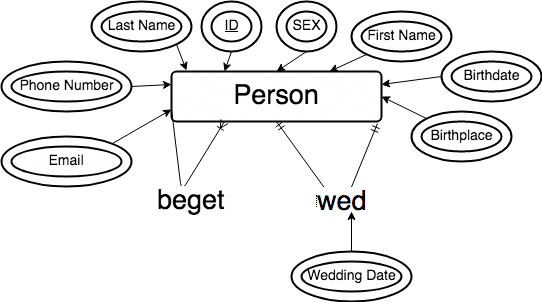
\includegraphics[width=\linewidth]{figs/entity.png}
        \caption{Entity-Relation Database Diagram}
        \label{fig:er}
    \end{figure}
    The Entity-Relation diagram has been converted to tables in the following way:
    \begin{enumerate}
        \item{The main entity \textit{Person} is presented as a table incorporating all information about people in a family tree. It
            has ID field as a primary key. }
        \item{The $1-1$ relation "wed" encodes the marital bonds between people, and $1-N$ relation "beget" encodes the parental
            bonds. They both are represented as separate tables, which contain the edges of a family tree. The former is also made to
            be symmetrical, i.e. $wed(x, y) \iff wed(y, x)$, which allows for more coherent reasoning about genealogy. Symmetry means that
            each record in the table 'wed' is doubled and reversed after being inserted.}
    \end{enumerate}
    Each row is loaded from DB and stored in the next sub-component, \textit{Model}, as a graph data structure. The model defines all
    the necessary methods to work with this graph, including \textit{Breadth-First Search} algorithm that is used to find to minimal
    path between two vertices.

    The \textit{Visualiser} then renders this tree inside a predefined rectangular region, which can be further scaled and moved by
    the special camera class. This class implements a lightweight version of a 2D graphical engine.

    \subsection{Virtual Assistant}
    After careful considerations, we settled on a list of English questions that our virtual assistant, named \textit{Ami}, can answer.
    This list is rich enough to satisfy any user and, at the same time, short enough to allow an actual implementation.
    Observe, that the list actually defines a \textit{infinite} amount of potential questions by including special
    \texttt{<reference>} part, which we define by again using convenient Bacus-Naur notation:
    \begin{align*}
        \text{\textbf{reference}} &::= \text{\textbf{name}} | \text{my \textbf{relative}} |
        \text{my \textbf{relative}s' \textbf{relative}} | \text{\textbf{relative} of \textbf{reference}} | \text{I} | \text{me} |
        \text{myself} \\
        \text{\textbf{relative}} &::= \text{\textbf{basic}} | \text{uncle} | \text{brother} | ... \\
        \text{\textbf{basic}} &::= \text{parents} | \text{parent} | \text{son} | ...
    \end{align*}
    Where \textbf{relative} stands for an \textit{image} of the dictionary $\omega$, \textbf{name} for the full name of a person and
    \textbf{basic} for all primal kinship terms.

    \begin{enumerate}
        \item{How is \texttt{<reference>} related to \texttt{<reference>}?}
        \item{How am I related to \texttt{<reference>}?}
        \item{Who is \texttt{<reference>}?}
        \item{Who is (a or an) \texttt{<relative>} of \texttt{<reference>}?}
        \item{Where \texttt{<reference>} (was or were) born?}
    \end{enumerate}
    As we can see, questions in this list have a coherent and static structure that can be parsed by machine, thus allowing us to take
    the most straightforward approach and implement them directly hard-coded string constants.

    Besides questions, Ami also accepts KISP queries that it channels to the Interpreter. For example, in order to query
    all females in genealogy one need to send the following message to Ami:
    \begin{verbatim}
    (filter (lambda (p) (= 'FEMALE' (attr p 'sex'))) people)
    \end{verbatim}
    Due to the incredibly versatile nature of our programming language, we can confidently say that there is no ineffable queries.
    Therefore, a user can always express himself at least in KISP, if not in English.

    Secondly, Ami can perform various auxiliary commands, such as:
    \begin{enumerate}
        \item{'Show [me] \texttt{<reference>}.' This command will center the view of a family tree on the specific person that is
            mentioned in the \texttt{<reference>}. If there are many persons, Ami will choose the first one. It is useful when we want
            to quickly locate a particular relative in a big tree.}
        \item{'Load filename.lisp', this command reads the specified file and executes its content as KISP source code. It may be of
            use when we need to quickly introduce new functions and definitions.}
    \end{enumerate}

    Finally, we must note that Ami is a \textit{context-free} assistant, which means that it takes into account only the very last
    message of the user. However, there is an important exception to this rule: if a user sends a message for the first time
    referring to himself, Ami will ask who he is, because there is no such information available by default. Context awareness of the
    virtual assistant is an interesting topic for future research, as well as considering different channels of user input, such as
    voice recognition.

    \subsection{KISP Interpreter}
    For the implementation of the KISP language we chose the most straightforward approach: firstly parse the source code, secondly,
    construct an AST, then perform an evaluation of that tree starting from its leaves, and finally output the result of the
    evaluation. However, in order to expedite this process, we introduced a caching mechanism, which remembers what terms yields to
    what results. Experienced user can manipulate this mechanism by the following commands:
    \begin{enumerate}
        \item{\texttt{Flush} completely removes all entries from cache table.}
        \item{\texttt{Set cache} enables caching mechanism.}
        \item{\texttt{Set nocache} disables caching mechanism.}
    \end{enumerate}
    Cache table automatically updates each time new definition is introduced or an old reference is redefined.

    For example, let’s evaluate the following terms:
    \begin{verbatim}
        (define ego (person ’John Smith’))
        (= ego ego)
        (define ego (person 'John Doe’))
        (= ’Doe’ (attr ego ’last name’))
    \end{verbatim}
    The last term will be correctly evaluated to \texttt{true}, since the result of the term \texttt{ego} was automatically
    updated in the cache table.

    This concludes the implementation chapter.

\section{Query Examples}
In this section we will demonstrate how one can use KISP to perform various queries in a genealogical tree. Particularly, we
focus our attention on statements that express kinship terms.

Let's start with a simple task of selecting people based on a certain boolean condition. Suppose we want to query only those, who
have at least one child. This can be accomplished as follows:
\begin{verbatim}
(filter (lambda (p) (< 0 (count (children p)))) people)
\end{verbatim}
Here we iterate through the list of all people in a tree and take only those, on who defined lambda predicate evaluated to
\texttt{true}. The number of children for a particular person is calculated by counting elements of the list \texttt{(children
p)}.

The next task is to select all husbands, that is, all men who are married. This can be done in two ways: either select only
males and then discard all bachelors, or combine the two operations together in a single boolean predicate using \texttt{and}
clause:
\begin{verbatim}
(filter (lambda (p) (not (= void (spouse p))))
            (filter (lambda (p) (= 'MALE' (attr p 'sex')))
            people))
(filter (lambda (p) (and (= 'MALE' (attr p 'sex'))
                         (not (= vacant (spouse p)))))
    people)
\end{verbatim}
The advantage of the second approach is that the list \texttt{people} will be iterated only once.

Now to the more advanced queries; suppose that the term \texttt{ego} stands for the user's node in an ancestry, and he wants to
know how many cousins he has:
\begin{verbatim}
(define parents (lambda (p) (join (mother p) (father p))))
(define cousins
    (lambda (p) (children (children (parents (parents p))))))
(- (count (cousins ego)) 1)
\end{verbatim}
This is where the expressive power of KISP truly comes into play. Although \texttt{cousins} is not a standard KISP function, we
can easily implement it using kinship framework of KISP, which successfully utilizes the structure of natural kinship terms.
Moreover, notice how the function \texttt{parents} is expressed. Since a parent is either a mother or a father, it corresponds to
the formal kinship term $(mother \vee father)$, which is implemented as a \textit{join} of two or more lists. And because every
cousin is a grand-child of one's grandparents, it corresponds to:
\begin{align*}
    (son \vee daughter)(son \vee daughter)(mother \vee father)(mother \vee father)
\end{align*}
The last decrement was made because in this scheme the \texttt{ego} itself will be included to the resulting list.

Finally, temporal queries can be expressed with the help of the type \textit{Date}. For instance, if we need to know, who, among our
relatives, was born during the WWII, we just need to evaluate:
\begin{verbatim}
(define WWII-start (date '01.09.1939'))
(define WWII-end (date '02.09.1945'))
(filter (lambda (p) (during (attr p 'birthdate') WWII-start WWII-end))
    people)
\end{verbatim}
The type \textit{Date} provides all the necessary functions for working with temporal information.

Because KISP is Turing-complete and inherits LISP's capabilities of meta-programming, one can easily extend it with any
functionality that one wants.
